\documentclass[a4paper]{llncs}

%\usepackage{amssymb}
%\setcounter{tocdepth}{3}
\usepackage{graphicx}

%\usepackage[linesnumbered,ruled,vlined]{algorithm2e}


\usepackage[colorlinks=true,
urlcolor=blue,
citecolor=blue,
linkcolor=blue,
           bookmarks=false,
           bookmarksnumbered,
           linktocpage=true
           ]{hyperref}

\usepackage{url}

% \urldef{\mailsa}\path|{alfred.hofmann, ursula.barth, ingrid.haas, frank.holzwarth,|
% \urldef{\mailsb}\path|anna.kramer, leonie.kunz, christine.reiss, nicole.sator,|
% \urldef{\mailsc}\path|erika.siebert-cole, peter.strasser, lncs}@springer.com|    
% \newcommand{\keywords}[1]{\par\addvspace\baselineskip
% \noindent\keywordname\enspace\ignorespaces#1}

%\usepackage{tikz}
%\usepackage{aeguill}
%\usepackage{tikzscale}
%\usepackage{filecontents} 
\usepackage{subfig}
\usepackage[font=small]{caption}

\usepackage{times}
\usepackage{courier}

\usepackage{color}

\newcommand{\mypara}[1]{\vspace{4pt}\noindent\textbf{#1}}
\newcommand{\mytt}[1]{\ensuremath{\mathtt{#1}}}

%% PM Define authornote command for comments
\newcommand{\authornote}[2] {
    \begin{center}
        \framebox{
            {\begin{minipage}[t]{0.9\linewidth}
                \color{red}
                \raggedright  \textbf{[#1]}~ \scriptsize #2 \normalsize
            \end{minipage}}
    }
    \end{center}
}

\usepackage{listings}

\lstset{
basicstyle=\tiny\ttfamily,
breaklines=true,
frame=single
}



\begin{document}

\mainmatter  % start of an individual contribution

% first the title is needed
\title{DataONE: A Data Federation with Provenance Support}

% \author{Yang Cao\inst{1} \and Christopher Jones\inst{2} \and V\'ictor Cuevas-Vicentt\'in\inst{3} \and Steve Aulenbach\inst{4} \and Matthew B.\ Jones\inst{2} \and Bertram Lud\"ascher\inst{1} \and Timothy McPhillips\inst{1} \and Paolo Missier\inst{5} \and  Christopher Schwalm\inst{6} \and Peter Slaughter\inst{2} \and Dave Vieglais\inst{2} \and Lauren Walker\inst{2} \and Yaxing Wei\inst{7}}

\author{Yang Cao\inst{1},  Christopher Jones\inst{2},  V\'ictor Cuevas-Vicentt\'in\inst{3}, Matthew B.\ Jones\inst{2},  Bertram Lud\"ascher\inst{1},  Timothy McPhillips\inst{1},  Paolo Missier\inst{4},   Christopher Schwalm\inst{5},  Peter Slaughter\inst{2},  Dave Vieglais\inst{6},  Lauren Walker\inst{2}, Yaxing~Wei\inst{7}}


\institute{Library and Information Science, University of Illinois, Urbana-Champaign, IL\\
\and
National Center for Ecological Analysis and Synthesis, UCSB, CA \\
\and
Universidad Popular Aut\'onoma del Estado de Puebla, Mexico\\
\and
School of Computing Science, Newcastle  University, UK \\
\and
Woods Hole Research Center, Falmouth, MA \\
\and
University of Kansas, Lawrence, KS \\
\and
Environmental Sciences Division, Oak Ridge National Laboratory, TN 
}



%
% NB: a more complex sample for affiliations and the mapping to the
% corresponding authors can be found in the file "llncs.dem"
% (search for the string "\mainmatter" where a contribution starts).
% "llncs.dem" accompanies the document class "llncs.cls".
%

\toctitle{Lecture Notes in Computer Science}
\tocauthor{Authors' Instructions}
\maketitle


\begin{abstract}
  DataONE is a federated data network focusing on earth and environmental science data.  We demonstrate new provenance capabilities in the DataONE toolkit to facilitate reproducible research. A user ``Alice'', can annotate a (Matlab, R, etc.) script using the YesWorkflow (YW) tool to describe the underlying workflow or \emph{prospective} provenance. After Alice has run the script, the result files, script, prospective provenance, and \emph{retrospective} provenance, represented in the ProvONE provenance model, are bundled into an OAI-ORE compliant data package and uploaded to the DataONE network. A second user (``Bob'') discovers Alice's package and uses her data in his own analysis. We show that Bob's results, once published through DataONE, link back to Alice's outputs via unique identifiers. Thus, a third user (``Charlie'') who browses DataONE discovers the full provenance of Bob's results, all the way back to Alice's original contributions.  DataONE provenance systems enable reproducible research and facilitate proper attribution of scientific results transitively across generations of derived data products.  \end{abstract}

% \keywords{We would like to encourage you to list your keywords within
% the abstract section}



\section{Introduction}

Scientific workflow \emph{provenance} is valuable in computational science. Provenance can help scientists to understand their own work and share their work with others while maintaining attribution. We refer to two types of provenance: \emph{prospective} and \emph{retrospective} provenance, where the former refers to a specification of a data transformation process \cite{Freire2008}, and the latter refers to the derivations that account for the actual outcomes of one execution of the process.

DataONE (Data Observation Network for Earth) is a federated data network and a sustainable cyberinfrastructure for open, persistent, robust, and secure access to well-described and easily discovered Earth observational data~\cite{dataone}. The primary goals of DataONE are: (i) data discovery, access, integration and synthesis;  (ii) education and training, building community; and (iii) data sharing. The DataONE infrastructure consists of three principal components:

\mypara{(1) Member Nodes} are existing or new data repositories that support the DataONE Member Node API.  Tier-1 Member Nodes (MN) implement anonymous, read-only access to data and metadata and enable discovery of all objects available on the MN, with low level descriptions of each object, object retrieval by identifier, and activity reporting. MNs also provide science metadata and relationships between metadata and data using resource maps \cite{oaiore} to facilitate discovery.  MNs can also implement higher tiers of the DataONE API, including authenticated and restricted data access (Tier-2), write access to storage resources (Tier-3), and replication of data from other nodes (Tier-4).


\mypara{(2) Coordinating Nodes} (CN) serve the coordination and discovery needs of the network. Services of a CN include network-wide indexing of data objects, coordination of data replication between MNs, mirrored content of \emph{science metadata} (detailed descriptions of science data objects and collections) and \emph{system metadata} (low level metadata, e.g., data type, size, ownership, location) that are extracted from data files in the MNs.


\mypara{(3) Investigator Toolkit.} The Investigator Toolkit (ITK) contains developer tools that enable programmatic interaction with DataONE infrastructure through a REST service API exposed by the CNs and MNs. Python and Java libraries are available for application developers, and DataONE support is present in scientific analysis tools such as Matlab and R.


The DataONE infrastructure was released for public use in 2012 and supports identifier resolution, content search and retrieval, an infrastructure for federated identity management, and replication service for both data and metadata.

%\subsection*{DataONE Search}

\mypara{DataONE Search} is a web-based application that lets users seamlessly and efficiently discover publicly accessible data packages within the DataONE federated network of Member Node repositories. It allows users to search across space (geographical region), time, and using a set of keywords. Users sign in to DataONE Search using ORCID credentials, Google accounts, or institutional accounts. DataONE enables new user features like provenance-based browsing as part of its search facility.

%\authornote{PM}{I suggest explaining why we are introducing Search here -- saying for instance that DataONE enables new user features like provenance-based browsing as part of its search facility.\\
%Also `` other facets and to refine the results using further parameters. '' is a bit vague, I would remove this part.}

The software has been designed to facilitate rapid iteration and deployment of new features and to take full advantage of future capabilities offered by upcoming versions of the core cyberinfrastructure. Notable among these is the \emph{provenance information} within search and discovery. In the next section, we will demonstrate new DataONE provenance tools and the visualization of provenance with DataONE Search.


\section{Demonstration Description}  \label{demo}

In this demonstration we describe two features related to provenance. 
The first is an API for capturing \textit{retrospective} provenance from R \cite{recordr} and Matlab \cite{matlabdataone} script executions, called \emph{Run Manager}.
The second is a script annotation tool, which we call YesWorkflow \cite{yesworkflow}, designed to help developers and users better understand the structure and intent of a script.
%DataONE has developed a API , and contributed to the development of to provide an improved understanding of a script in terms of its user-declared workflow structure and system-recorded file I/O. 


%\authornote{PM}{The automatic capture of the latter is transparent to scientists and provides medium-grained\footnote{unlike the fine-grained provenance captured, e.g., by noWorkflow \cite{nw14}} provenance by focusing on file I/O events.
%orphan sentence, but it seems to try and say too much -- is it necessary?}

We introduce the provenance and search features of DataONE by means of an example involving three earth scientists who interact through a DataONE MN, as shown in Fig.~\ref{fig0}. First Alice generates and publishes new grass fraction maps from observational data, eg. water, air temperature~\cite{MsTMIP-model-driver-data-set}. Then Bob uses Alice's data to run further analysis~\cite{MsTMIP-model-output-data-set}, i.e., on grassland water use efficiency and publishes it back to a DataONE MN. Finally, Charlie, a DataONE user, examines the provenance of Bob's published data to determine its suitability for his own use.

\subsection{Alice's Data Generation}

%\begin{figure}
%\centering   
%\subfloat[YesWorkflow annotations example used in Alice's script which annotate a block of code with input and output information \label{yw}]{%
%      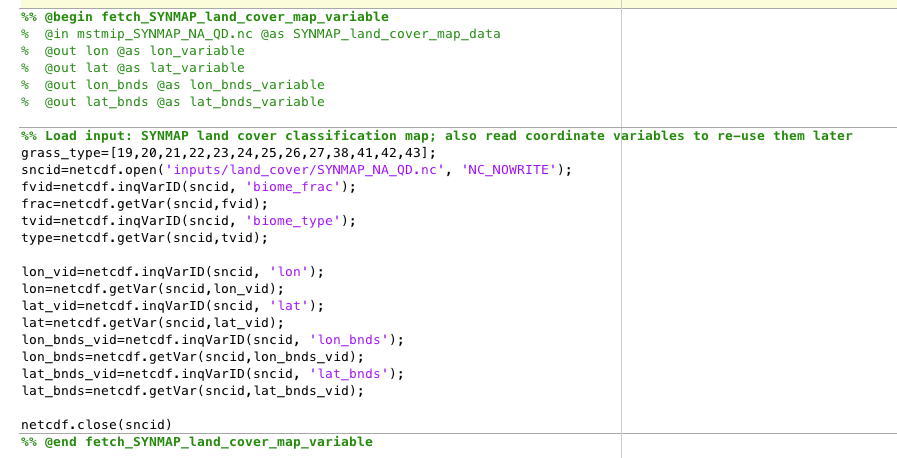
\includegraphics[width=0.5\textwidth, height=2in]{yw-annotations}
%  }
%\subfloat[Alice calls the record() function to record a run for her script \label{record-snapshot}]{%
%      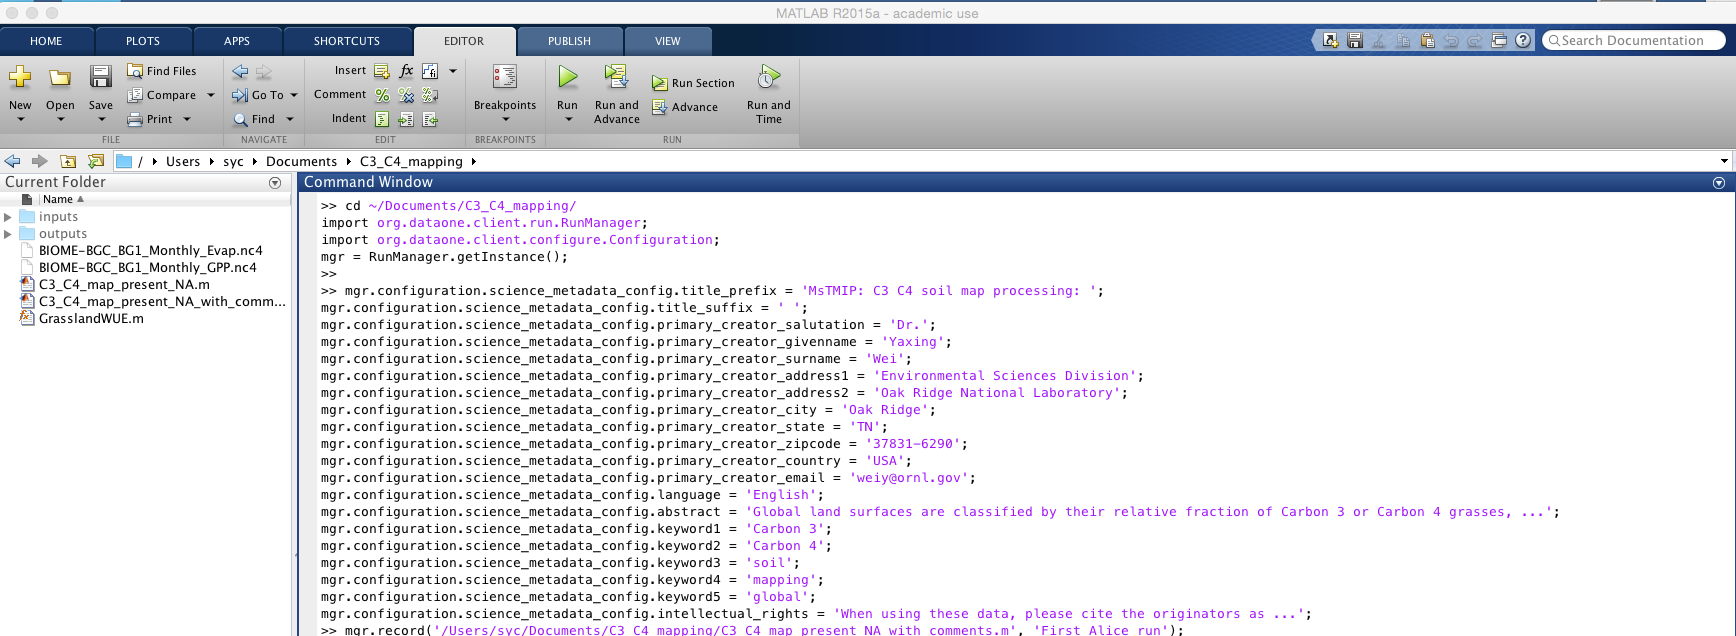
\includegraphics[width=0.5\textwidth, height=2in]{record_Alice_run}
% }
% \\
% \subfloat[Alice calls the view() function to check the recorded execution information \label{view-snapshot}]{%
%      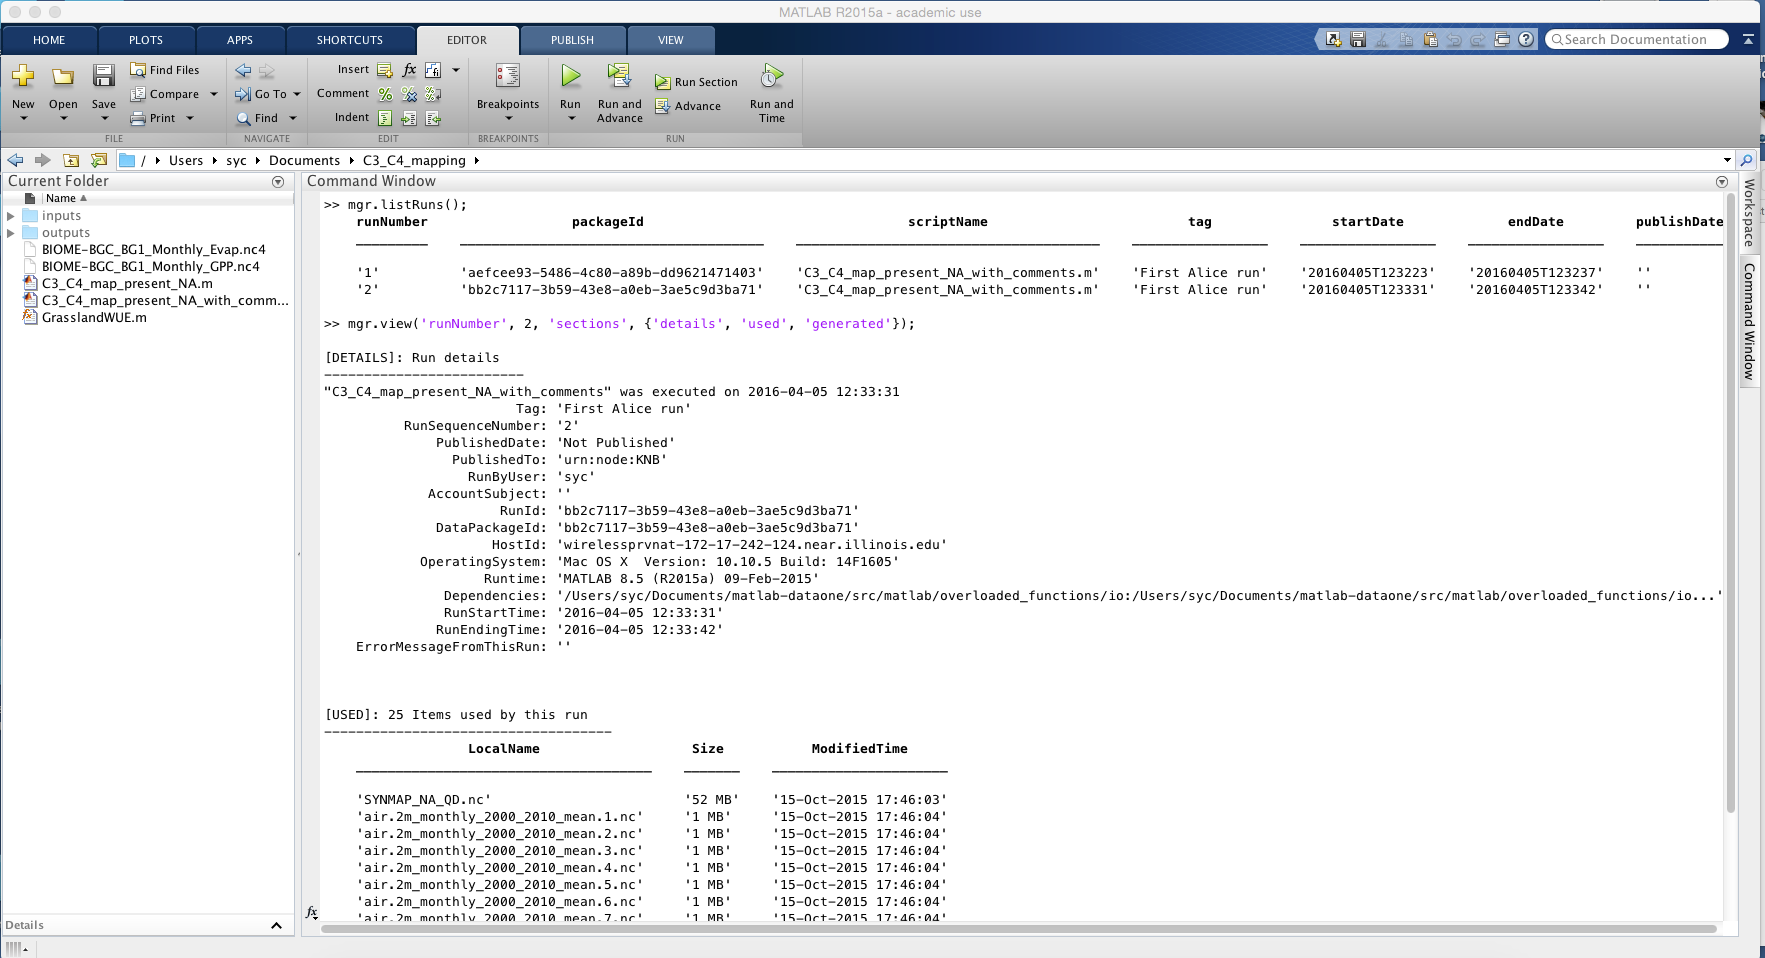
\includegraphics[width=0.5\textwidth, height=2in]{view_Alice_run}
% }
% \subfloat[Alice calls the publish() function to share her execution and data with others to DataONE network \label{publish-snapshot}]{%
%      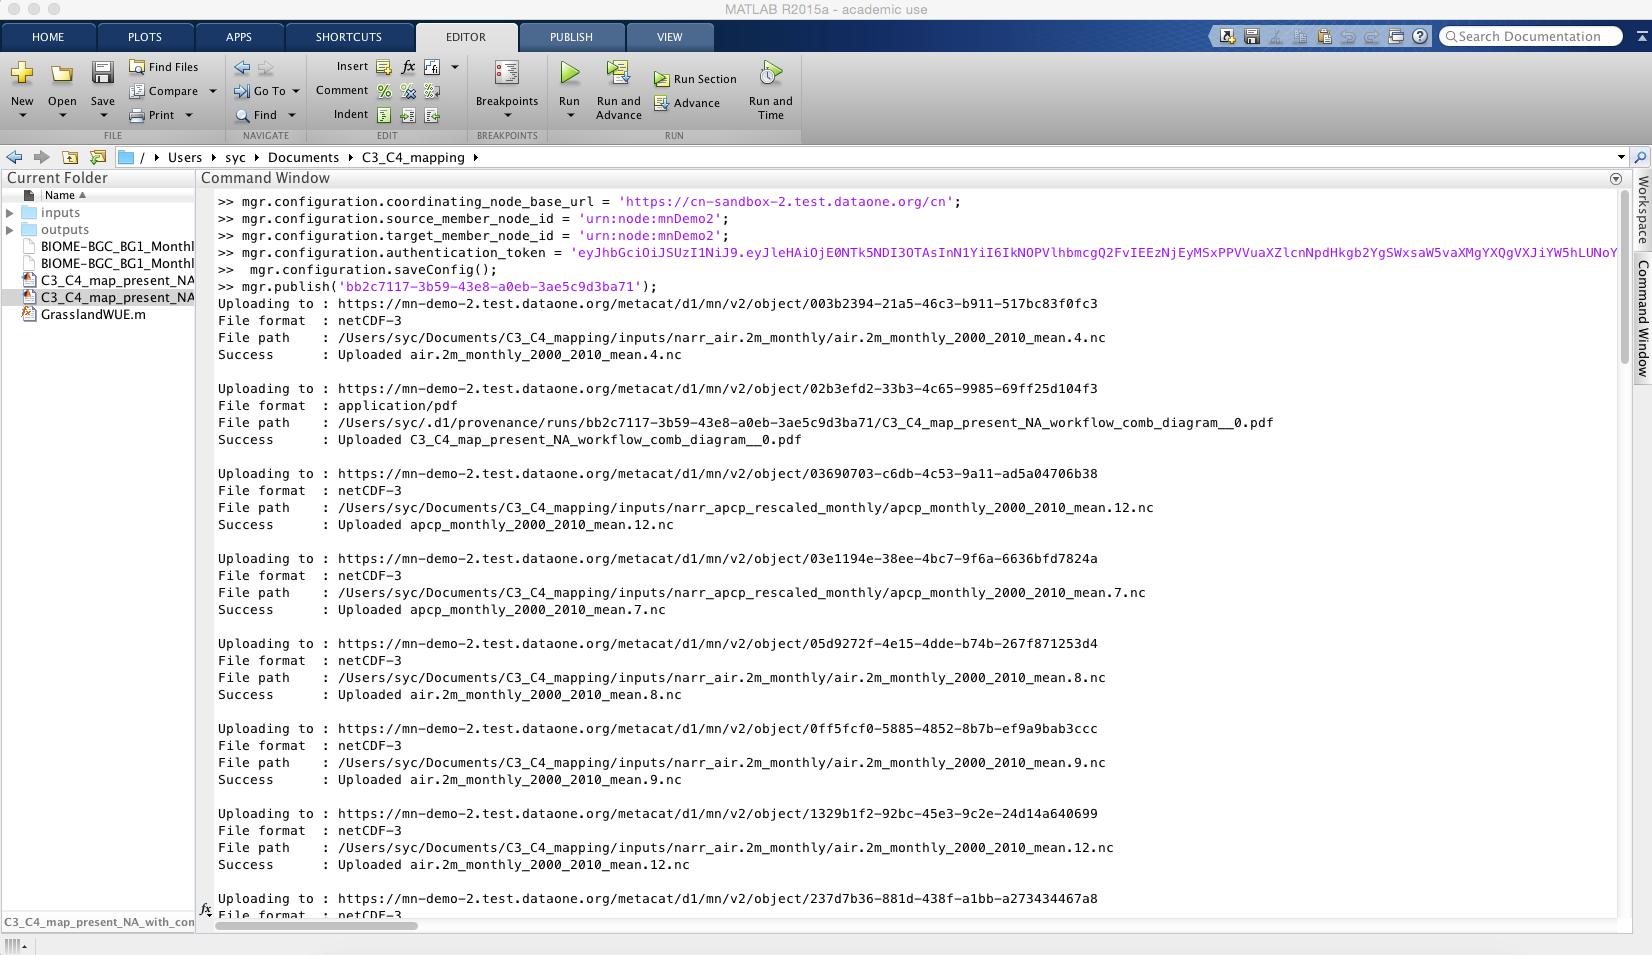
\includegraphics[width=0.5\textwidth, height=2in]{publish_Alice_run}
% }
% \caption{Snapshots when Alice uses DataONE Provenance tool to annotate her script steps, record the execution of her script, view the details for one run, and publish her run to the DataONE network.}
%\label{fig0}
%\end{figure}

%\begin{figure}[t] \centering 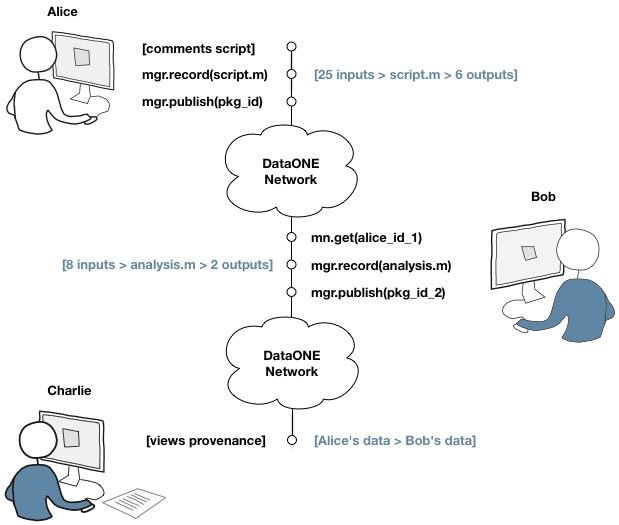
\includegraphics[width=0.5\textwidth]{alice-bob-charlie-sequence} \caption{Run Manager Demonstration: (1) Alice runs \mytt{script.m} with the DataONE Run Manager to create data package $P_A$, which she publishes to the DataONE network; (2) Bob later finds and downloads Alice's data, uses it in his \mytt{analysis.m}, creating and then publishing package $P_B$; (3) Charlie searches DataONE, finds Bob's $P_B$, and recognizes its dependence on Alice's $P_A$.}  \label{fig0} \end{figure}


As shown at the top of Fig.~\ref{fig0}, Alice has developed a script for producing Carbon3/Carbon4 soil maps.  She uses the YesWorkflow (YW) tool to mark-up the script and expose the underlying workflow view (i.e., prospective provenance) that is inherent in her soil mapping code as shown in Fig.\ref{yw-graph}. 

\begin{figure}[t] \centering 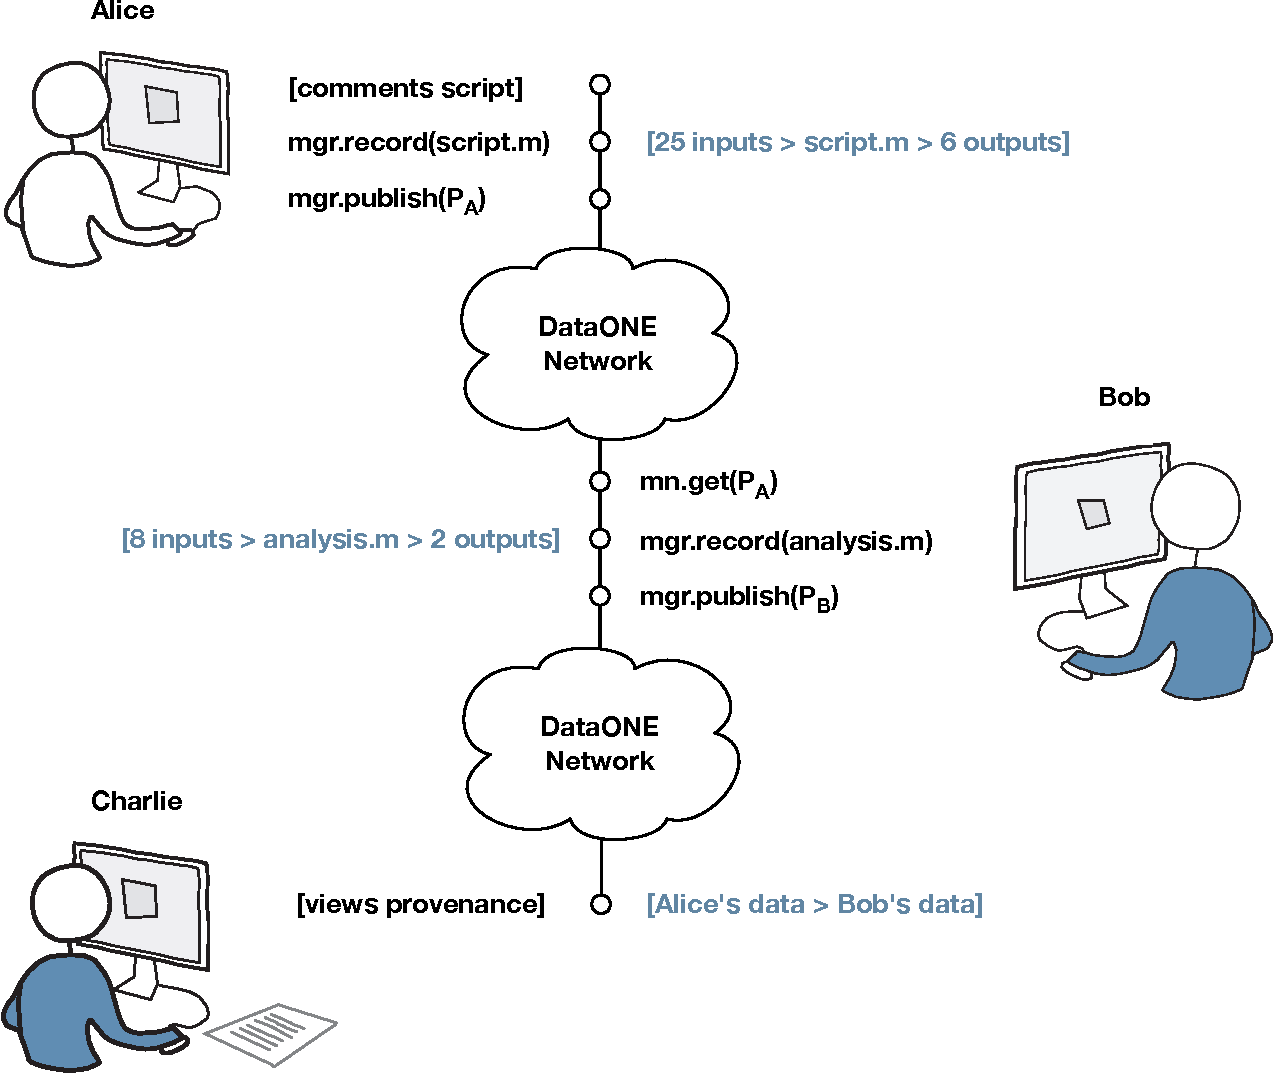
\includegraphics[width=0.6\textwidth]{figs/alice-bob-charlie-sequence-crop} \caption{Run Manager Demonstration: (1) Alice runs \mytt{script.m} with the DataONE Run Manager to create data package $P_A$, which she publishes to the DataONE network; (2) Bob later finds and downloads Alice's data, uses it in his \mytt{analysis.m}, creating and then publishing package $P_B$; (3) Charlie searches DataONE, finds Bob's $P_B$, and recognizes its dependence on Alice's $P_A$.}  \label{fig0} \end{figure}

\begin{figure}[!h] \centering 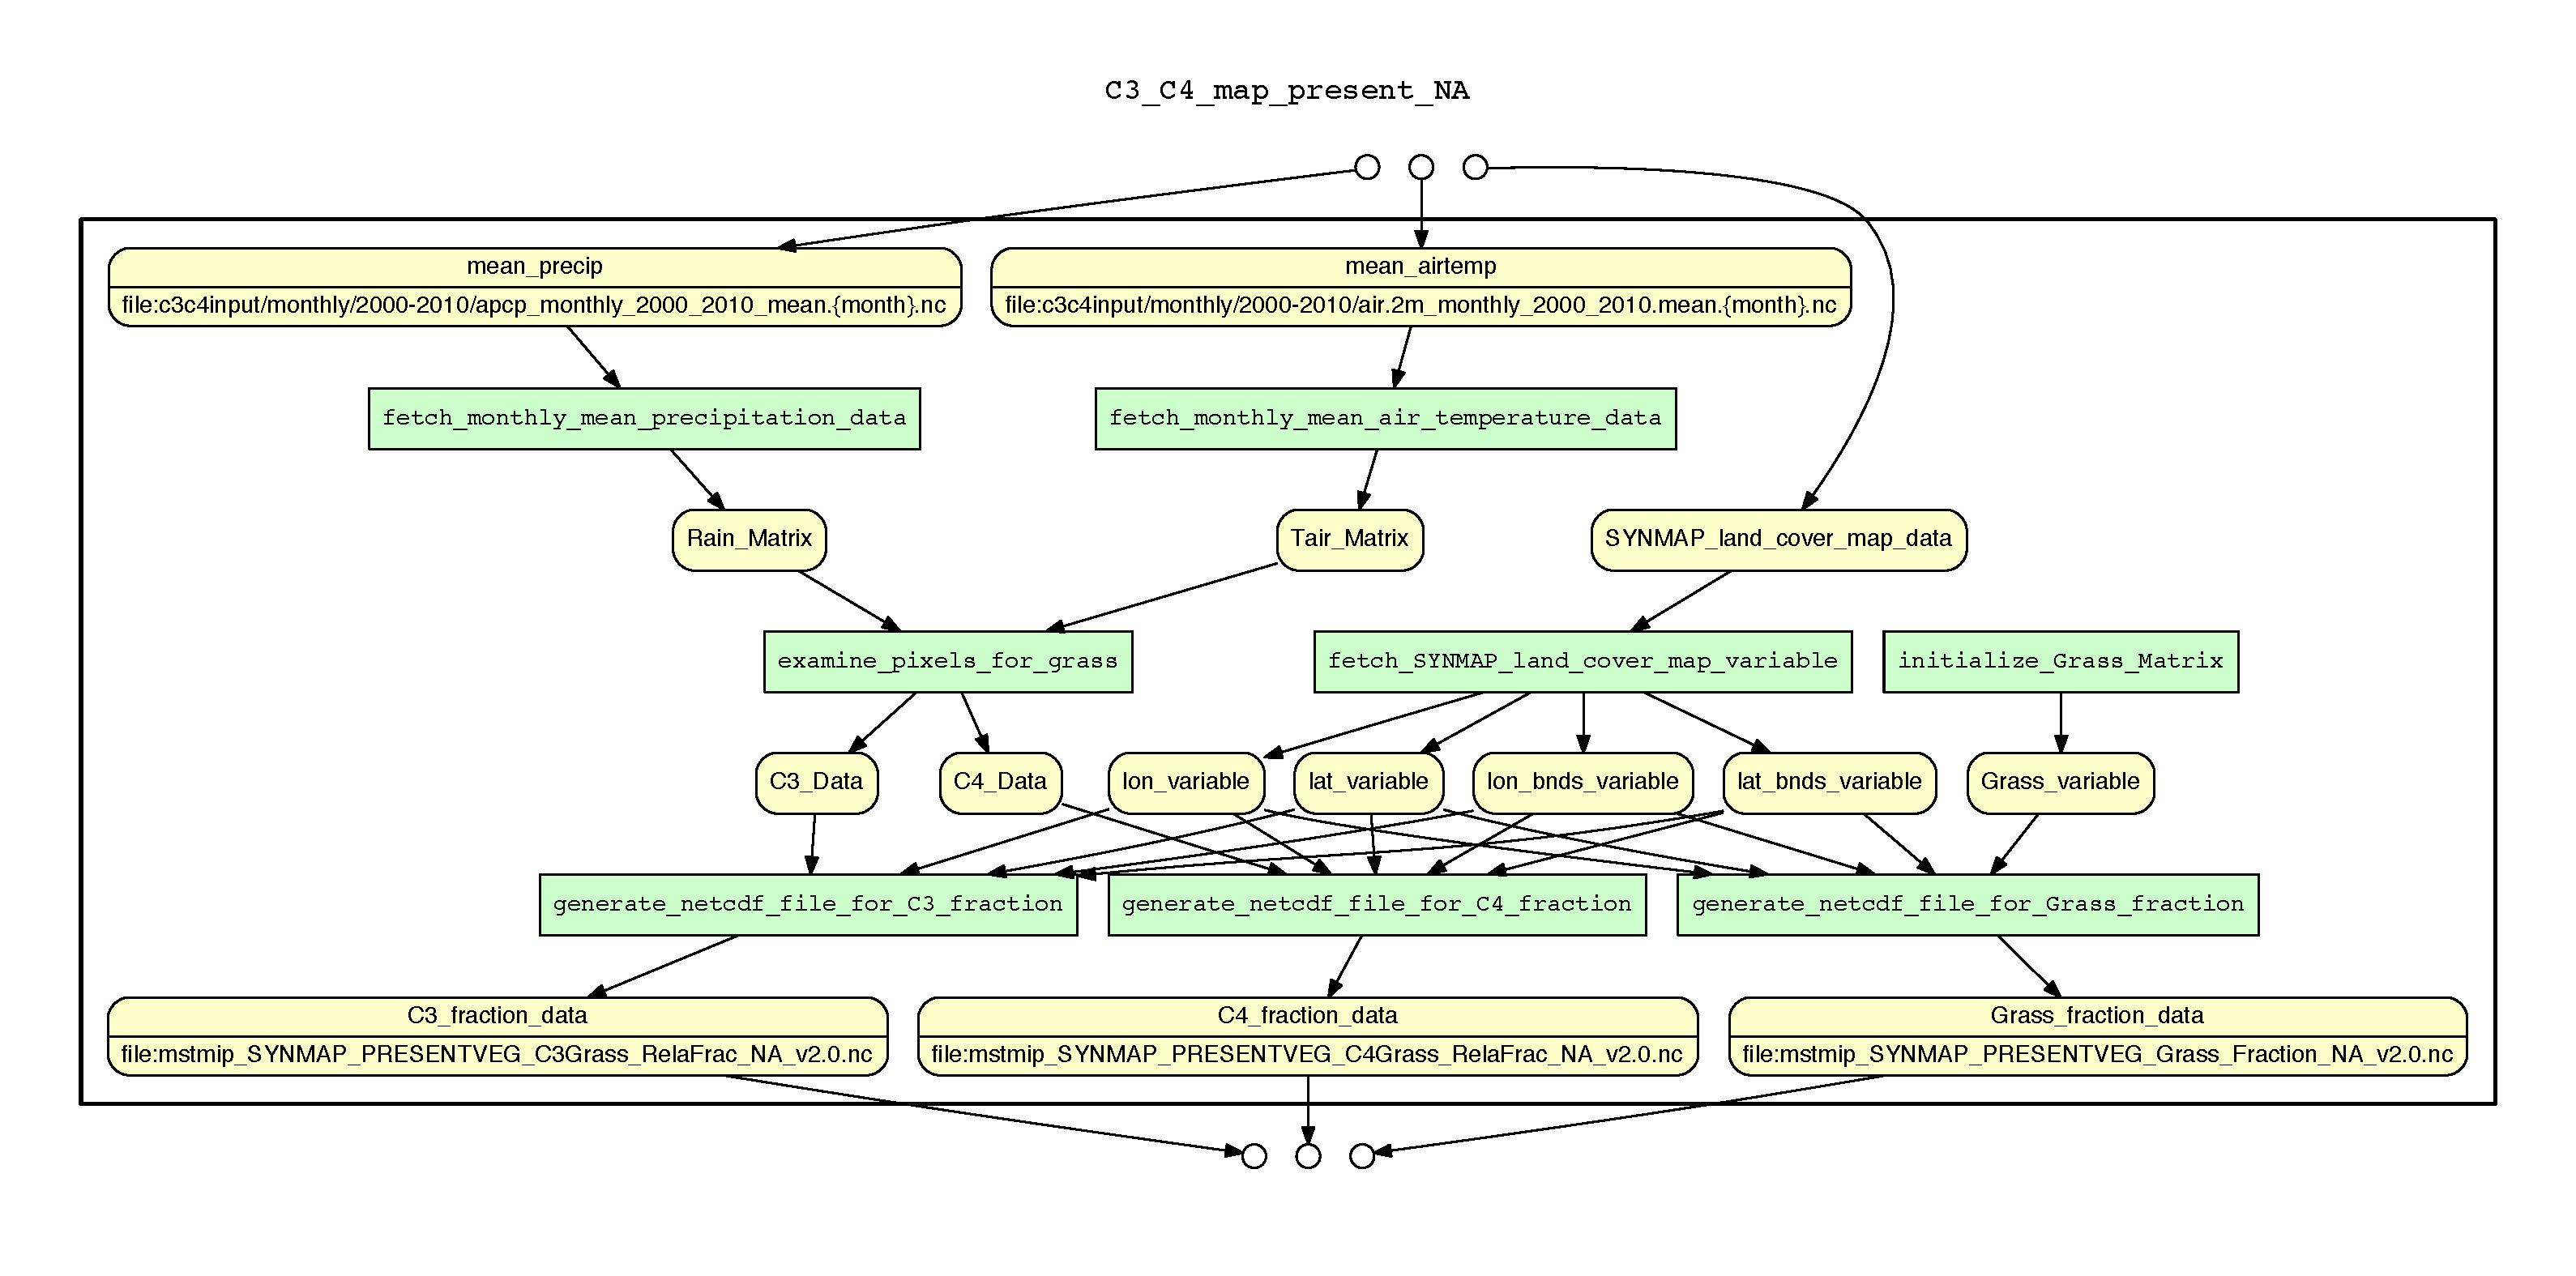
\includegraphics[width=1.05\textwidth]{figs/C3_C4_map_present_NA_workflow_comb_diagram} \caption{A combined view of the YesWorkflow model for Alice's soil processing scripts.}  \label{yw-graph} \end{figure}

%\authornote{PM}{need a ref here?  and a figure with the graph produced by YW on this script would be really useful to bring this part to life!}


By using the \emph{Run Manager} to run her script, Alice not only obtains the expected results, but she also captures their provenance, compliant with DataONE's ProvONE data model. 
ProvONE~\cite{provone} is an extension of the W3C PROV-O~\cite{prov-o} standard for representing provenance, and includes specializations for representing both retrospective provenance about the runtime execution and prospective provenance about the structure and flow of the analytical script or workflow.
%
At the end of the experimentation phase, Alice is ready to publish her results to a DataONE MN. 
To do so, she uses the  DataONE Matlab tool to automatically generate a DataONE-compliant data package in OAI-ORE format, including the ProvONE provenance document, the script itself, and its YW-generated workflow view. Partial ProvONE provenance statements included in the uploaded Alice's data package are provided in List~\ref{list1} of the Appendix.

%\begin{figure}[!h] \centering 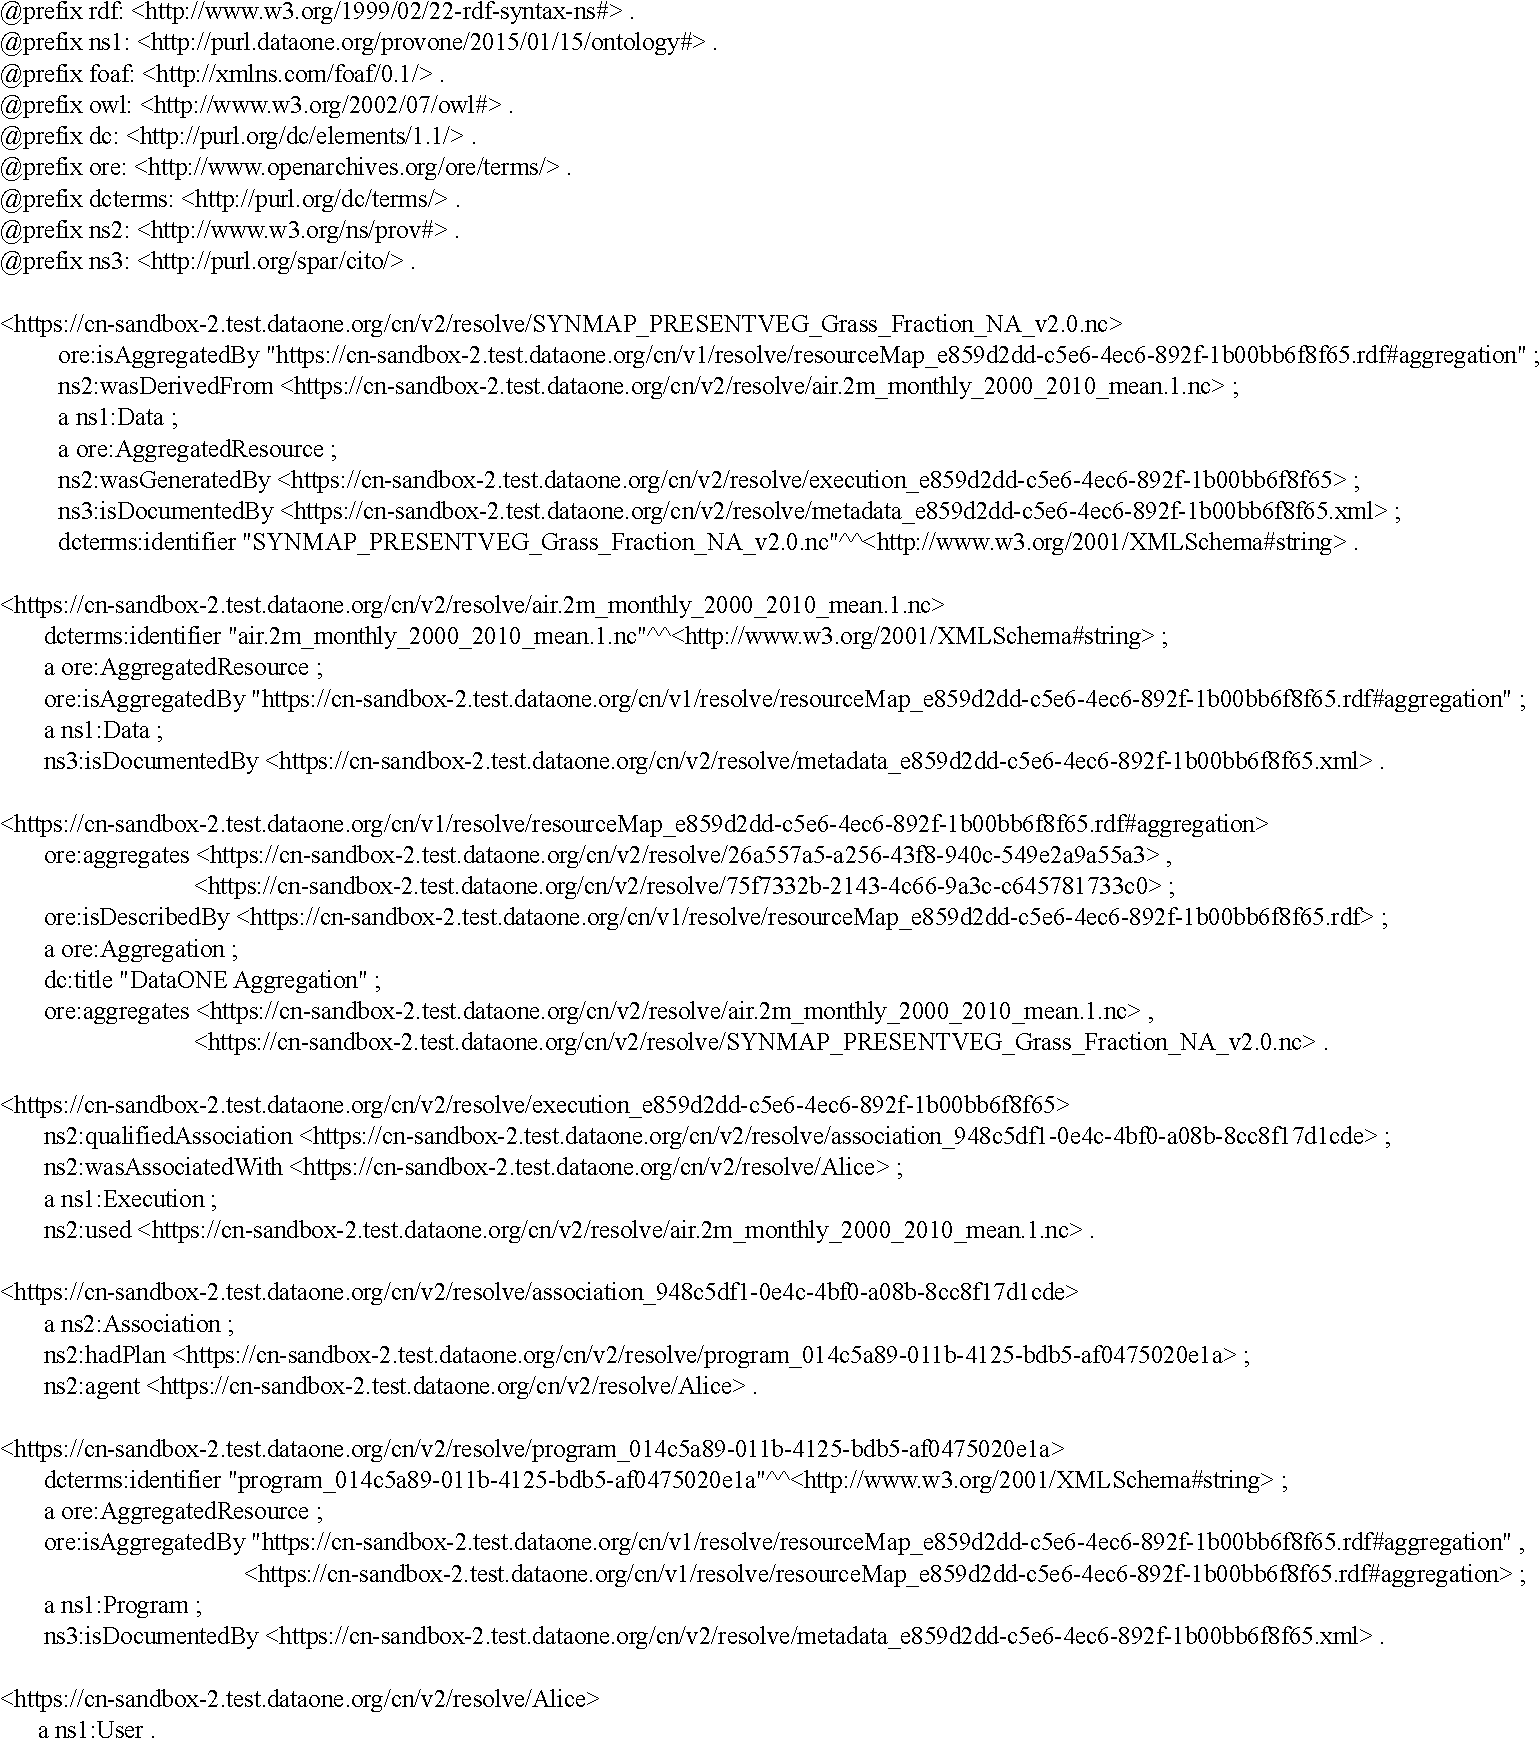
\includegraphics[width=1.7\textwidth]{figs/alice-ttl} \caption{ProvONE provenance statements included in the uploaded Alice's data package}  \label{list1} \end{figure}

Moreover, a YW-MATLAB module~\cite{yw-matlab} was developed to answer prospective and retrospective queries from provenance captured by YW and Run Manager. It contains a YW module and command line tools for interacting with the DataONE MATLAB RunManager~\cite{matlabdataone}. These tools make the recorded run-time data provenance available to YW so that this retrospective provenance information can be queried in terms of, and in combination with, the prospective provenance revealed by YW annotations in the MATLAB scripts.


\subsection{Bob's Data Reuse}

Bob's interaction with DataONE begins with a user interface search, i.e., using the keyword ``grass'', he discovers Alice's data package, amongst others. 
%\authornote{PM}{Why  is \cite{yaxing} cited here?}
He decides to use three NetCDF output data files which are part of the package, as input to his Grassland Water Use Efficiency Analysis script . 
Having identified the data of interest in the MN, Bob uses its public identifier \textit{id} to retrieve it and use it in his own code (GrasslandWUE.m).
Specifically, the \mytt{MemberNode.get}(session, id)  call, available from the Matlab Toolbox, not only correctly retrieves Alice's data package, but it also ensures that the download event is recorded as part of a new provenance document, associated to Bob's analysis.
%
Note that, should Bob create a new identifier when he downloads Alice's data, the link between two data packages would be broken, leading to a disconnect in provenance and requiring additional ``stitching'' operations~\cite{missing-link}.  

Instead, by retaining the same identifier throughout, the tool implicitly establishes a connection between Alice's work and Bob's, namely by adding a provenance statement of the form (Bob's\_execution, \emph{prov:used}, Alice's\_data\_id).
%\authornote{PM}{can you be completely explicit here?  it should look like used([\textbf{bob's script name as above}], id)}.
Bob then proceeds to operate on the data using the DatAONE Matlab just like Alice did, eventually publishing a new data package with his own results and their provenance.
At this point, the two provenance documents are physically disjoint, as they reside in different data packages, but they are logically connected, namely through the used() statement mentioned above.
As they are both indexed by the CN upon publication of the data package, this logical connection emerges automatically when a third party, such as Charlie in our example, explores one of the two data packages.


\subsection{Charlie's Visual Data Navigation}

%\authornote{PM}{Charlie discovers Bob's data packages on DataONE and is able to navigate back to the data that Bob used, i.e., Alice's data package depicted in Figure~\ref{fig2}~\cite{Katz,data-trajectories}.
%}

Charlie discovers Bob's data packages on DataONE and is able to navigate back to the data that Bob used, i.e., Alice's data package depicted in Fig.~\ref{fig2}~\cite{Katz,data-trajectories}. When he searches the DataONE network using the same keyword ``grass'' from the web search interface, two data packages are displayed as shown in Fig.~\ref{fig1}, namely Alice's and Bob's. 
One data package is created by ``Alice'' \cite{yaxing}, the other is created by ``Bob'' \cite{christopher}. 
%\authornote{PM}{I'm not quite sure how to fit Yaxing and Chris names here, it looks odd... why not replace Alice and Bob with Yaxing and Chris from the beginning?!?  and explain upfront that they are real scientists.}
%
Crucially, the provenance of the two datasets is now manifested visually along with their logical connection, as shown in the DataONE Search web UI for our demo site \cite{dataone-demo} (Fig.~\ref{fig2}) and is available to Charlie.
%
Specifically, Charlie can not only visualize the two data packages (Alice's is at the top and Bob's at the bottom), but he  is also aware of the derivation of Alice's data through Bob's script.
%

Provenance details for any input or output in the provenance graph can be viewed by clicking on the icon shown in the figure. DataONE Search also provides human language descriptions of how data are used or generated via the script and models, and provides navigation to ancestors and descendants in the data derivation chain. 
%
In this example, Charlie quickly learns that Alice's script (C3\_C4\_map\_present\_with\_comments.m) takes twenty-five input files and produces six outputs, shown on the left and right side of Alice's data package, respectively. The bottom three outputs in Alice's data package are the NetCDF data files that represent three different world map grids of percentage of grass types (C3 grass fraction, C4 grass fraction, and total grass fraction)~\cite{MsTMIP-model-driver-data-set}. In addition, a model graph is displayed at the intermediate layer that was generated by the YesWorkflow tool~\cite{yesworkflow}. Alice's used embedded YesWorkflow annotations to document her script. These annotations declare step by step how data are used and derived in the script. 

Similarly, from the provenance information associated with Bob's data package in Fig.~\ref{fig2}, we see that it takes eight inputs, and produces two visualizations~\cite{MsTMIP-model-output-data-set}. By viewing the details for each input, we can see that three of them are the outputs produced by Alice's data package.  


\begin{figure}[t]
\centering   
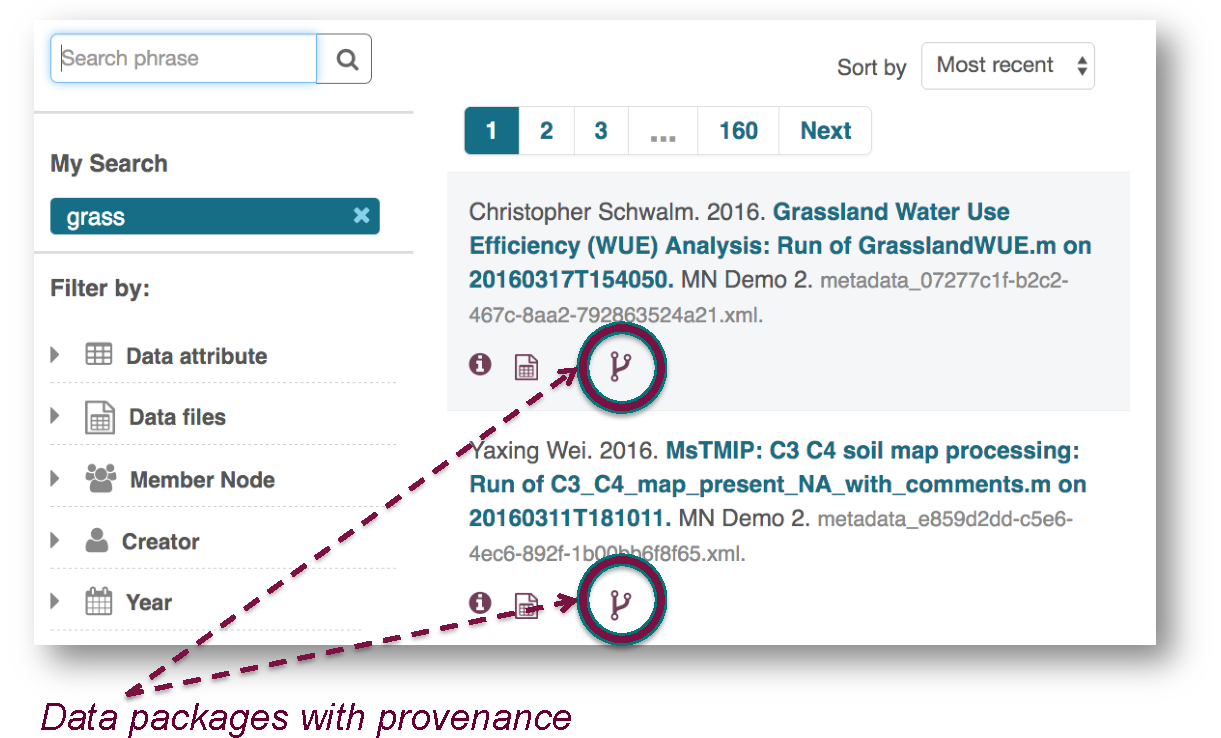
\includegraphics[width=0.7\textwidth]{figs/ab-crop}
\caption{DataONE Search result for keyword  ``grass'' (DataONE Search demonstration site). The ``fork'' icon indicates data packages having embedded provenance.}
\label{fig1}
\end{figure}



%Bob's data package \cite{christopher} created by DataONE provenance tool (Run Manager) is displayed at the bottom layer. When Bob browses Alice's data package on the DataONE Search site, he decides to use three NetCDF output data produced by Alice's work in his Grassland Water Use Efficiency Analysis script (GrasslandWUE.m). 
%
%In order to maintain the link between the outputs from Alice's data package to the inputs to Bob's package, Bob needs to use the same identifier in his script as Alice does. 
%

\begin{figure}[t]
\centering   
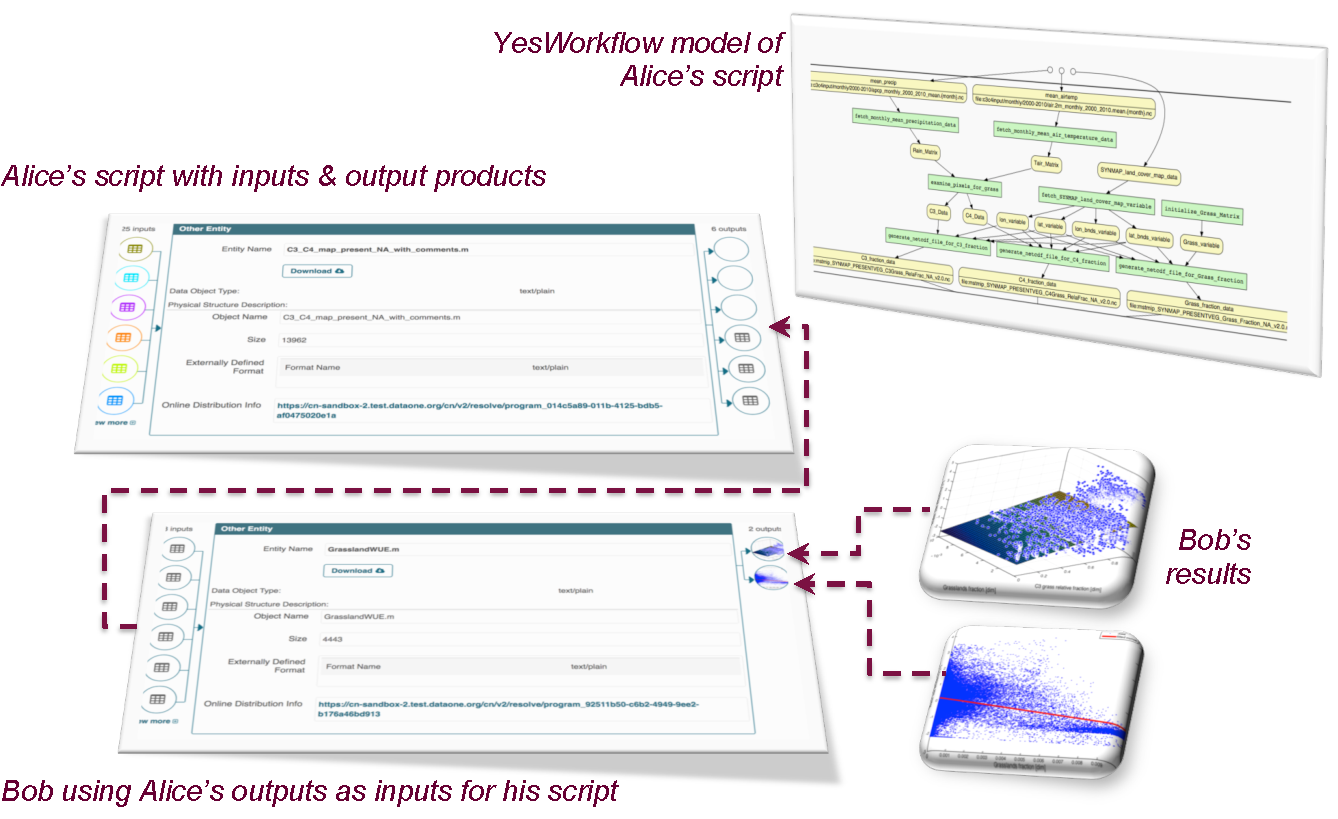
\includegraphics[width=0.8\textwidth]{figs/abc-crop}
\caption{Charlie's view on the DataONE demo site: (1) A YesWorkflow model for Alice's soil processing script; (2) Data lineage from Bob's results back through his script inputs to Alice's data package; (3) Two visualizations produced by Bob's water use efficiency analysis script.}
\label{fig2}
\end{figure}


\section{Discussion and Future Work}

This paper demonstrates a notable new feature (provenance capture and search) of DataONE. DataONE has released the DataONE Search for public use in November 2015, and the R and Matlab provenance tool to the public in 2016. 

Maintaining the link between Alice's work and Bob's subsequent work is worth discussion. Currently, Bob must use certain functions provided by DataONE to ensure the provenance link to Alice's work is correctly maintained. There are other possible ways to achieve the same goal. For example,  Bob might download Alice's data and manually add the links to Alice's work back into his data package before sharing via DataONE. A \emph{prov:was\_derived\_from} statement indicating that local data copy for Bob is derived from Alice's data could easily add, especially for historical data for which provenance was not captured at the time data were generated.  The new provenance tools described in this demonstration allow efficient capture of machine-parseable provenance information using analytical tools commonly used in the environmental sciences (e.g., Matlab), thereby significantly improving the replicability of research in the environmental sciences.


Future work of the current provenance tools include: (1) solve the broken link use case; (2) support more I/O functions; (3) handle complex scenarios such as multiple runs of a script and multiple users; (4) variable-level provenance capture warrants further investigation and efforts.


\bibliography{references}
\bibliographystyle{splncs03}

\newpage

\begin{appendix}
\section{Appendix}  

%\authornote{BL}{Could include the ProvONE statements as a verbatim environment instead of figure/PDF}

%\begin{figure}[h] \centering 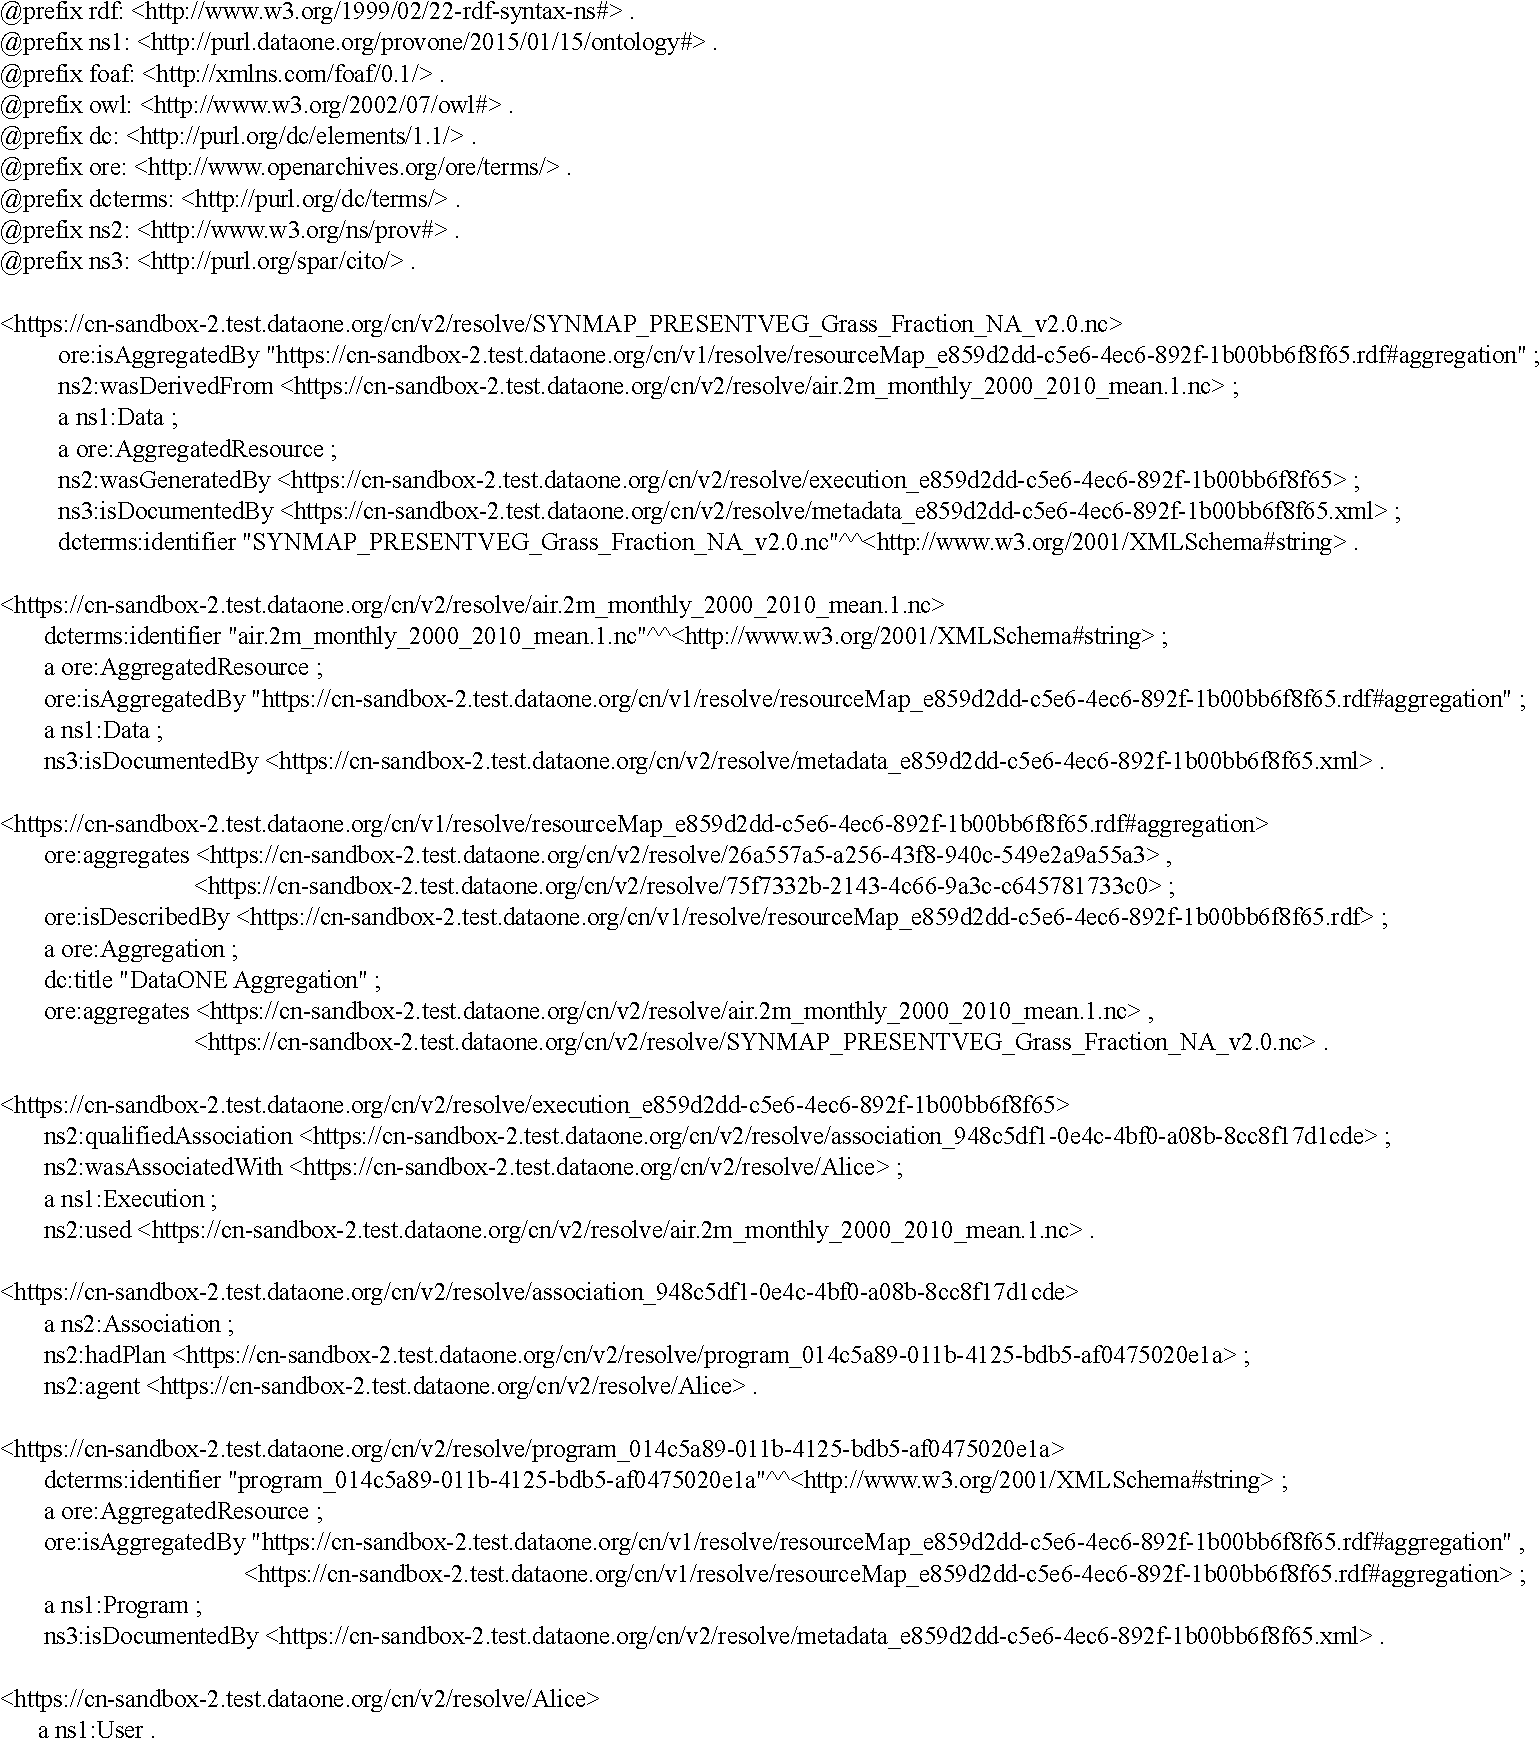
\includegraphics[width=0.8\textwidth]{figs/alice-ttl} 
%\caption{ProvONE provenance statements included in the uploaded Alice's data package}  \label{list1} \end{figure}

\begin{lstlisting} [caption=ProvONE provenance statements included in the uploaded Alice's data package, label=list1] 

@prefix rdf: <http://www.w3.org/1999/02/22-rdf-syntax-ns#> .
@prefix ns1: <http://purl.dataone.org/provone/2015/01/15/ontology#> .
@prefix foaf: <http://xmlns.com/foaf/0.1/> .
@prefix owl: <http://www.w3.org/2002/07/owl#> .
@prefix dc: <http://purl.org/dc/elements/1.1/> .
@prefix ore: <http://www.openarchives.org/ore/terms/> .
@prefix dcterms: <http://purl.org/dc/terms/> .
@prefix ns2: <http://www.w3.org/ns/prov#> .
@prefix ns3: <http://purl.org/spar/cito/> .

<https://cn-sandbox-2.test.dataone.org/cn/v2/resolve/SYNMAP_PRESENTVEG_Grass_Fraction_NA_v2.0.nc>
  ore:isAggregatedBy "https://cn-sandbox-2.test.dataone.org/cn/v1/resolve/resourceMap_e859d2dd-c5e6-4ec6-892f-1b00bb6f8f65.rdf#aggregation" ;
  ns2:wasDerivedFrom <https://cn-sandbox-2.test.dataone.org/cn/v2/resolve/air.2m_monthly_2000_2010_mean.1.nc> ;
  a ns1:Data ;
  a ore:AggregatedResource ;
  ns2:wasGeneratedBy <https://cn-sandbox-2.test.dataone.org/cn/v2/resolve/execution_e859d2dd-c5e6-4ec6-892f-1b00bb6f8f65> ;
  ns3:isDocumentedBy <https://cn-sandbox-2.test.dataone.org/cn/v2/resolve/metadata_e859d2dd-c5e6-4ec6-892f-1b00bb6f8f65.xml> ;
  dcterms:identifier "SYNMAP_PRESENTVEG_Grass_Fraction_NA_v2.0.nc"^^<http://www.w3.org/2001/XMLSchema#string> .

<https://cn-sandbox-2.test.dataone.org/cn/v2/resolve/air.2m_monthly_2000_2010_mean.1.nc>
  dcterms:identifier "air.2m_monthly_2000_2010_mean.1.nc"^^<http://www.w3.org/2001/XMLSchema#string> ;
  a ore:AggregatedResource ;
  ore:isAggregatedBy "https://cn-sandbox-2.test.dataone.org/cn/v1/resolve/resourceMap_e859d2dd-c5e6-4ec6-892f-1b00bb6f8f65.rdf#aggregation" ;
  a ns1:Data ;
  ns3:isDocumentedBy <https://cn-sandbox-2.test.dataone.org/cn/v2/resolve/metadata_e859d2dd-c5e6-4ec6-892f-1b00bb6f8f65.xml> .

<https://cn-sandbox-2.test.dataone.org/cn/v1/resolve/resourceMap_e859d2dd-c5e6-4ec6-892f-1b00bb6f8f65.rdf#aggregation> 
  ore:aggregates <https://cn-sandbox-2.test.dataone.org/cn/v2/resolve/26a557a5-a256-43f8-940c-549e2a9a55a3> , <https://cn-sandbox-2.test.dataone.org/cn/v2/resolve/75f7332b-2143-4c66-9a3c-c645781733c0> ;
  ore:isDescribedBy <https://cn-sandbox-2.test.dataone.org/cn/v1/resolve/resourceMap_e859d2dd-c5e6-4ec6-892f-1b00bb6f8f65.rdf> ;
  a ore:Aggregation ;
  dc:title "DataONE Aggregation" ;
  ore:aggregates <https://cn-sandbox-2.test.dataone.org/cn/v2/resolve/air.2m_monthly_2000_2010_mean.1.nc> , <https://cn-sandbox-2.test.dataone.org/cn/v2/resolve/SYNMAP_PRESENTVEG_Grass_Fraction_NA_v2.0.nc> .

<https://cn-sandbox-2.test.dataone.org/cn/v2/resolve/execution_e859d2dd-c5e6-4ec6-892f-1b00bb6f8f65>
  ns2:qualifiedAssociation <https://cn-sandbox-2.test.dataone.org/cn/v2/resolve/association_948c5df1-0e4c-4bf0-a08b-8cc8f17d1cde> ;
  ns2:wasAssociatedWith <https://cn-sandbox-2.test.dataone.org/cn/v2/resolve/Alice> ;
  a ns1:Execution ;
  ns2:used <https://cn-sandbox-2.test.dataone.org/cn/v2/resolve/air.2m_monthly_2000_2010_mean.1.nc> .

<https://cn-sandbox-2.test.dataone.org/cn/v2/resolve/association_948c5df1-0e4c-4bf0-a08b-8cc8f17d1cde>
  a ns2:Association ;
  ns2:hadPlan <https://cn-sandbox-2.test.dataone.org/cn/v2/resolve/program_014c5a89-011b-4125-bdb5-af0475020e1a> ;
  ns2:agent <https://cn-sandbox-2.test.dataone.org/cn/v2/resolve/Alice> .

<https://cn-sandbox-2.test.dataone.org/cn/v2/resolve/program_014c5a89-011b-4125-bdb5-af0475020e1a>
  dcterms:identifier "program_014c5a89-011b-4125-bdb5-af0475020e1a"^^<http://www.w3.org/2001/XMLSchema#string> ;
  a ore:AggregatedResource ;
  ore:isAggregatedBy "https://cn-sandbox-2.test.dataone.org/cn/v1/resolve/resourceMap_e859d2dd-c5e6-4ec6-892f-1b00bb6f8f65.rdf#aggregation" , <https://cn-sandbox-2.test.dataone.org/cn/v1/resolve/resourceMap_e859d2dd-c5e6-4ec6-892f-1b00bb6f8f65.rdf#aggregation> ;
  a ns1:Program ;
  ns3:isDocumentedBy <https://cn-sandbox-2.test.dataone.org/cn/v2/resolve/metadata_e859d2dd-c5e6-4ec6-892f-1b00bb6f8f65.xml> .

<https://cn-sandbox-2.test.dataone.org/cn/v2/resolve/Alice>
  a ns1:User .
\end{lstlisting}

\end{appendix}

\end{document}
